\section{Git areas}
\subsection{The stages of Git}
\begin{frame}[fragile]
    \frametitle{Different areas in git}
    \begin{figure}
        \begin{center}
            \ifnumequal{\aspectratio}{43}
            {
                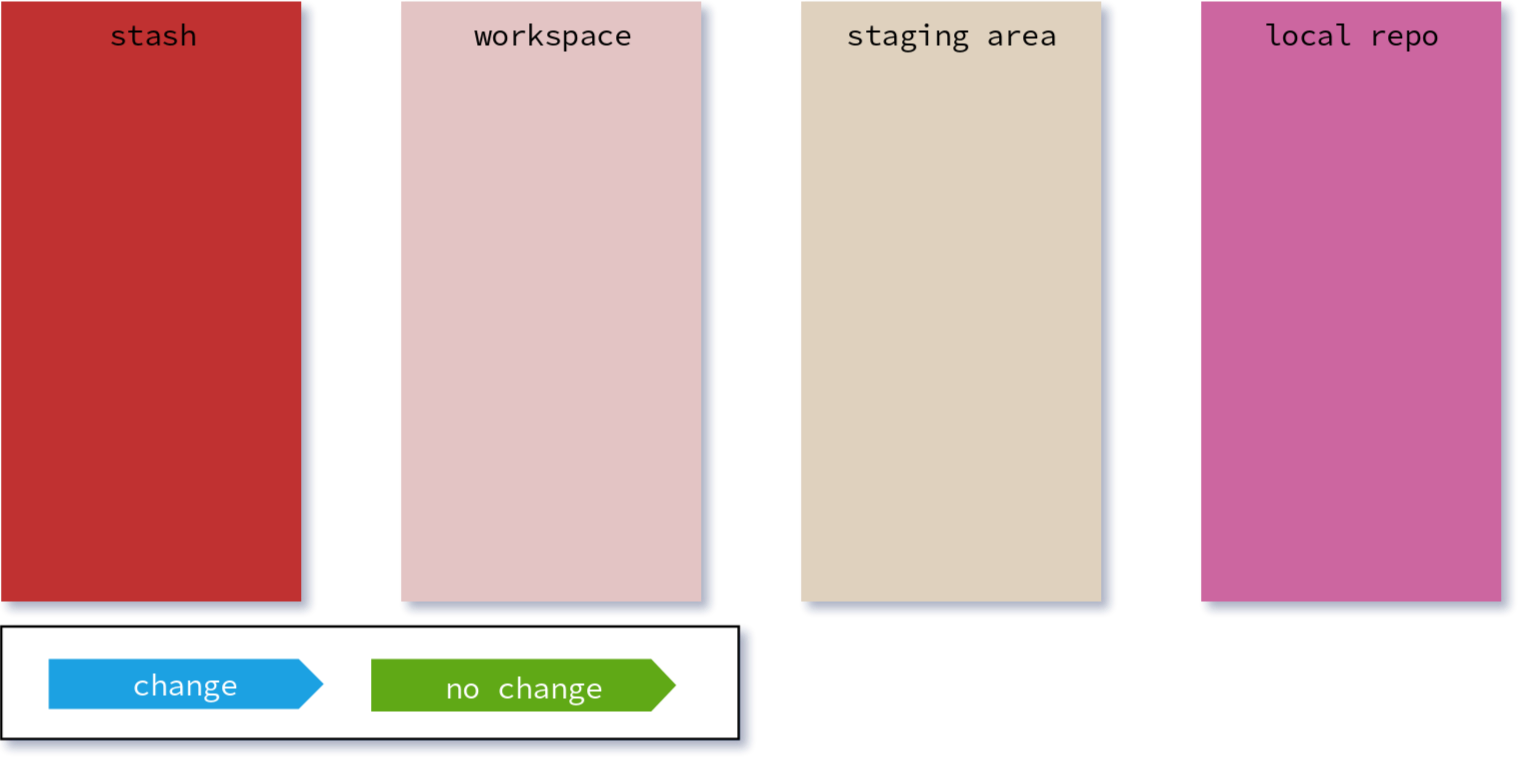
\includegraphics[width=1\textwidth,keepaspectratio]{./images/GitAreas.png}
            }
            {
                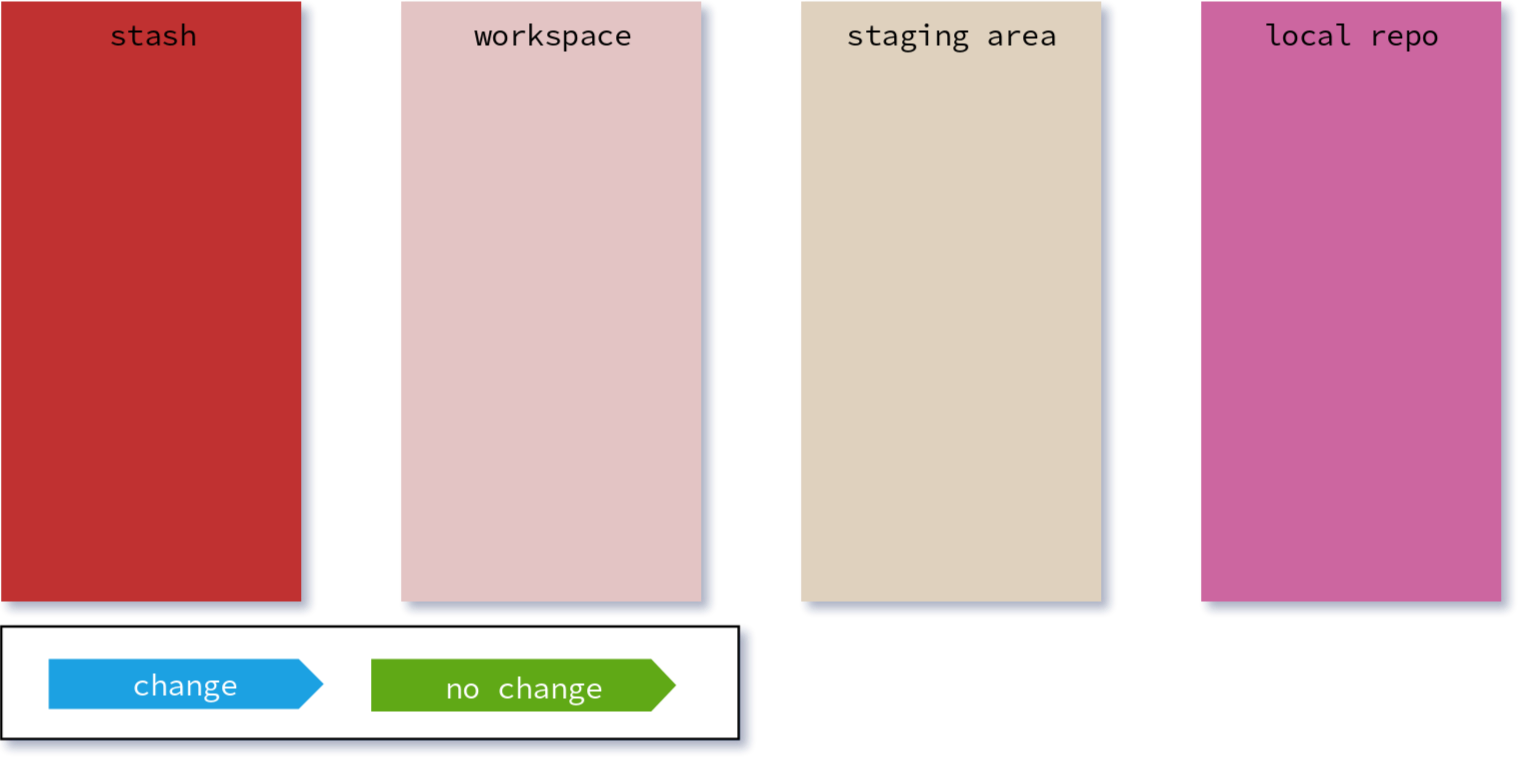
\includegraphics[height=0.75\textheight,keepaspectratio]{./images/GitAreas.png}
            }
            \caption{Areas in git}
        \end{center}
    \end{figure}
\end{frame}

\begin{frame}[fragile,noframenumbering]
    \frametitle{Git Workspace}
    \addtocounter{page}{-1}
    \begin{figure}
        \begin{center}
            \ifnumequal{\aspectratio}{43}
            {
                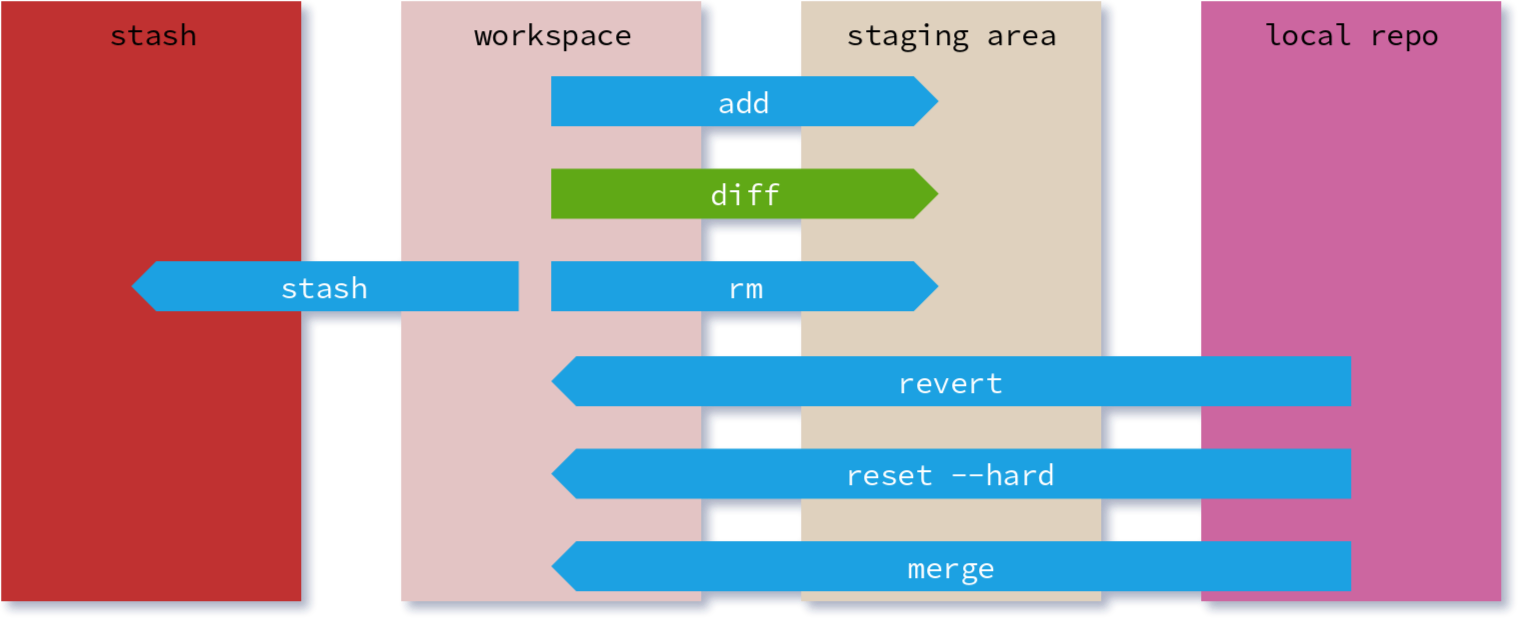
\includegraphics[width=1\textwidth,keepaspectratio]{./images/GitAreas-Workspace.png}
            }
            {
                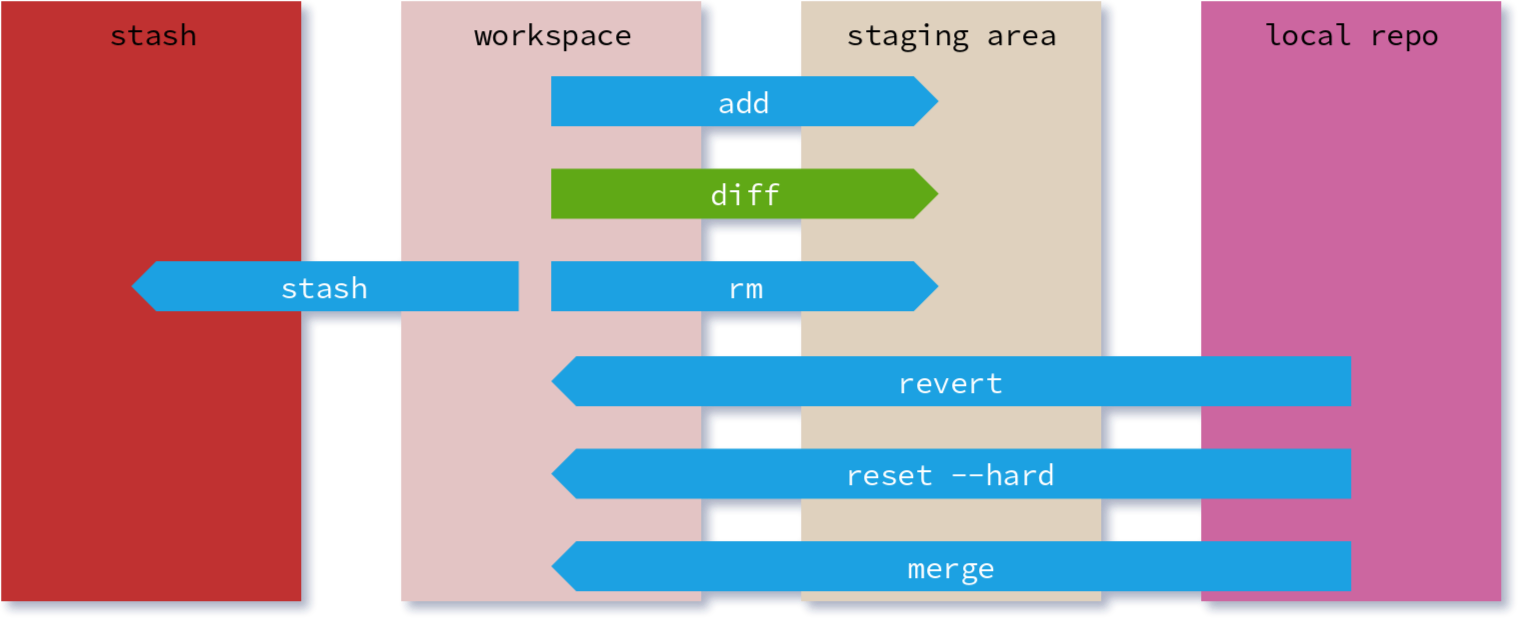
\includegraphics[height=0.75\textheight,keepaspectratio]{./images/GitAreas-Workspace.png}
            }
            \caption{Workspace area}
        \end{center}
    \end{figure}
\end{frame}

\begin{frame}[fragile,noframenumbering]
    \frametitle{Git Staging}
    \addtocounter{page}{-1}
    \begin{figure}
        \begin{center}
            \ifnumequal{\aspectratio}{43}
            {
                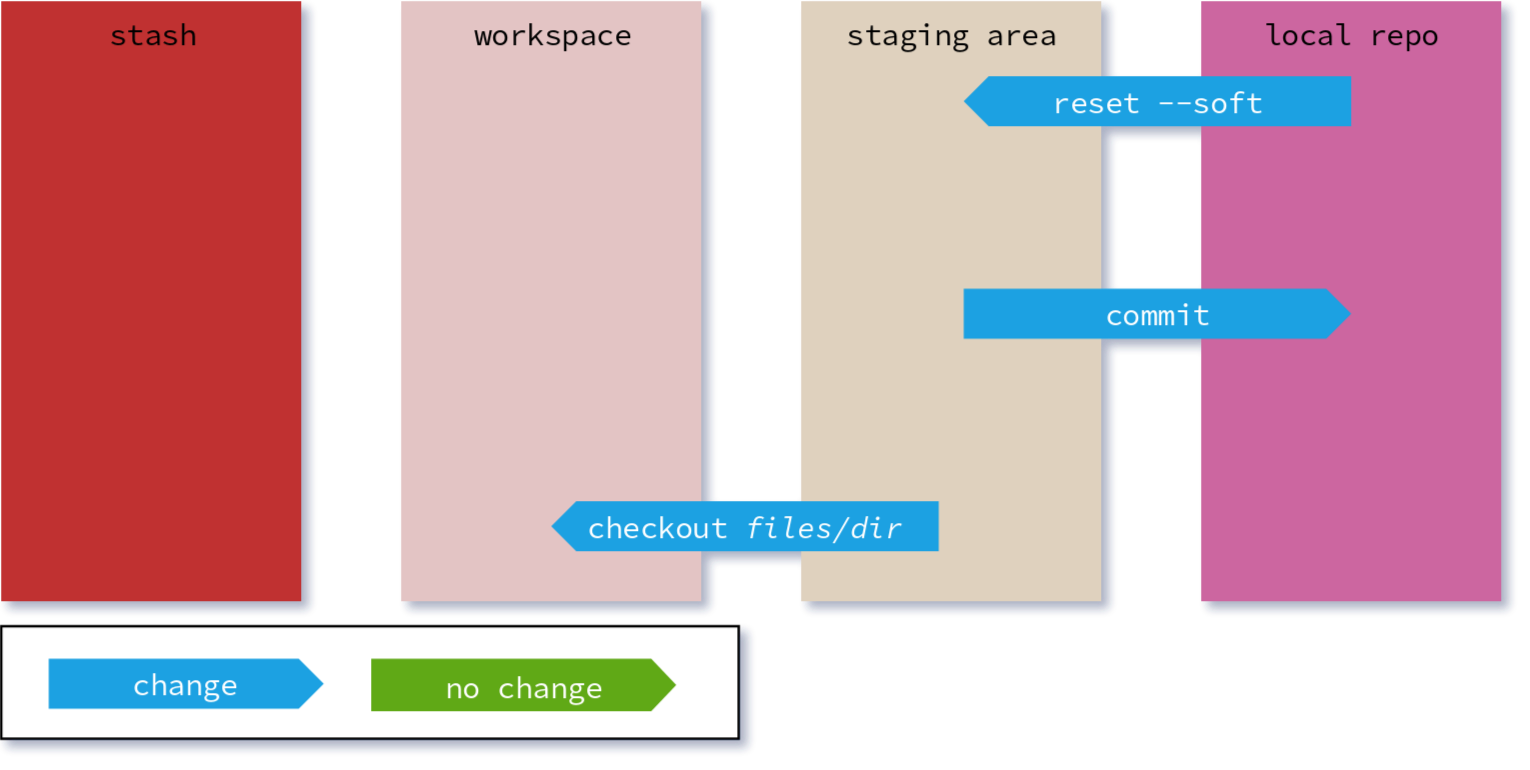
\includegraphics[width=1\textwidth,keepaspectratio]{./images/GitAreas-Staging.png}
            }
            {
                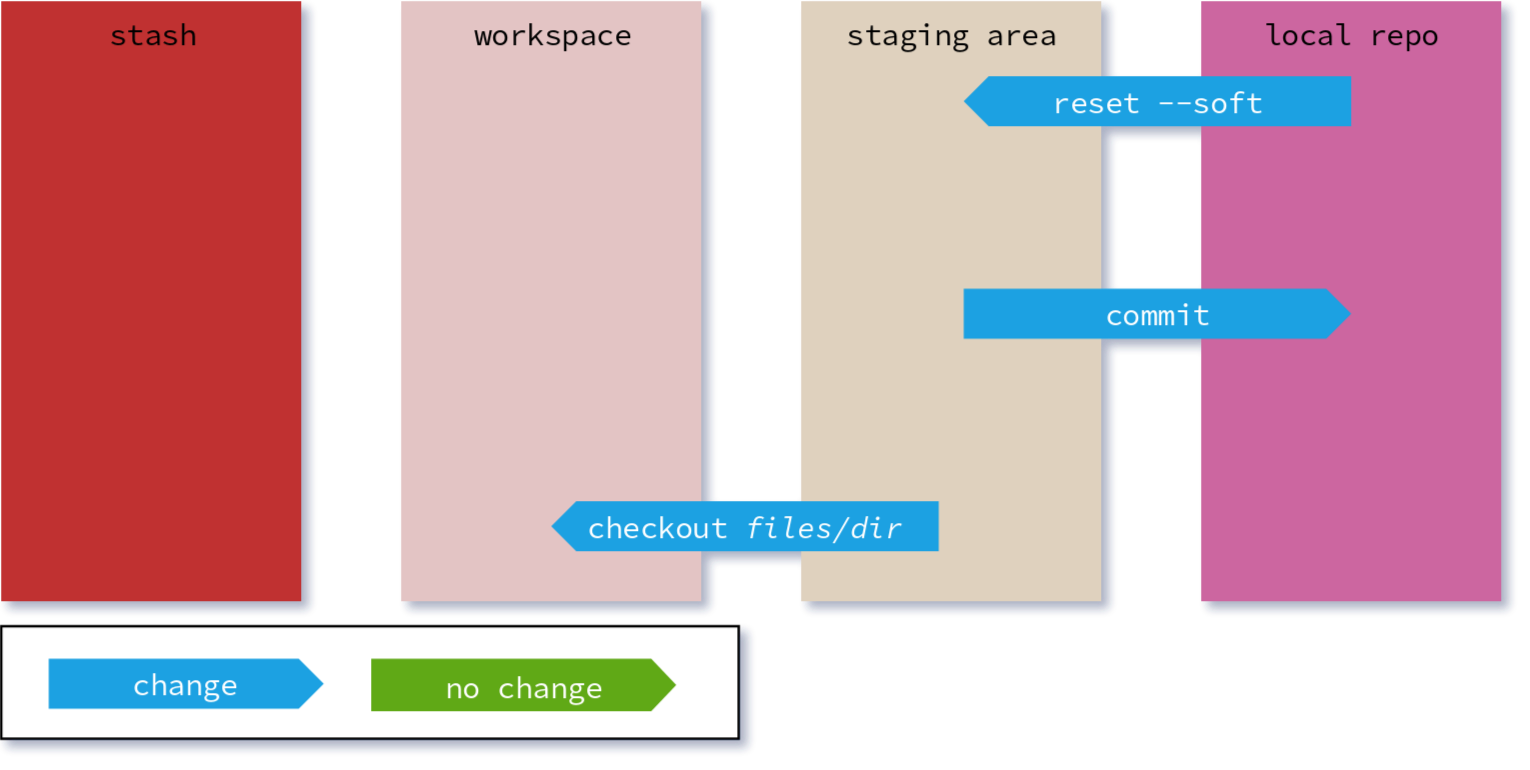
\includegraphics[height=0.75\textheight,keepaspectratio]{./images/GitAreas-Staging.png}
            }
            \caption{Staging area}
        \end{center}
    \end{figure}
\end{frame}

\begin{frame}[fragile,noframenumbering]
    \frametitle{Git local repository}
    \addtocounter{page}{-1}
    \begin{figure}
        \begin{center}
            \ifnumequal{\aspectratio}{43}
            {
                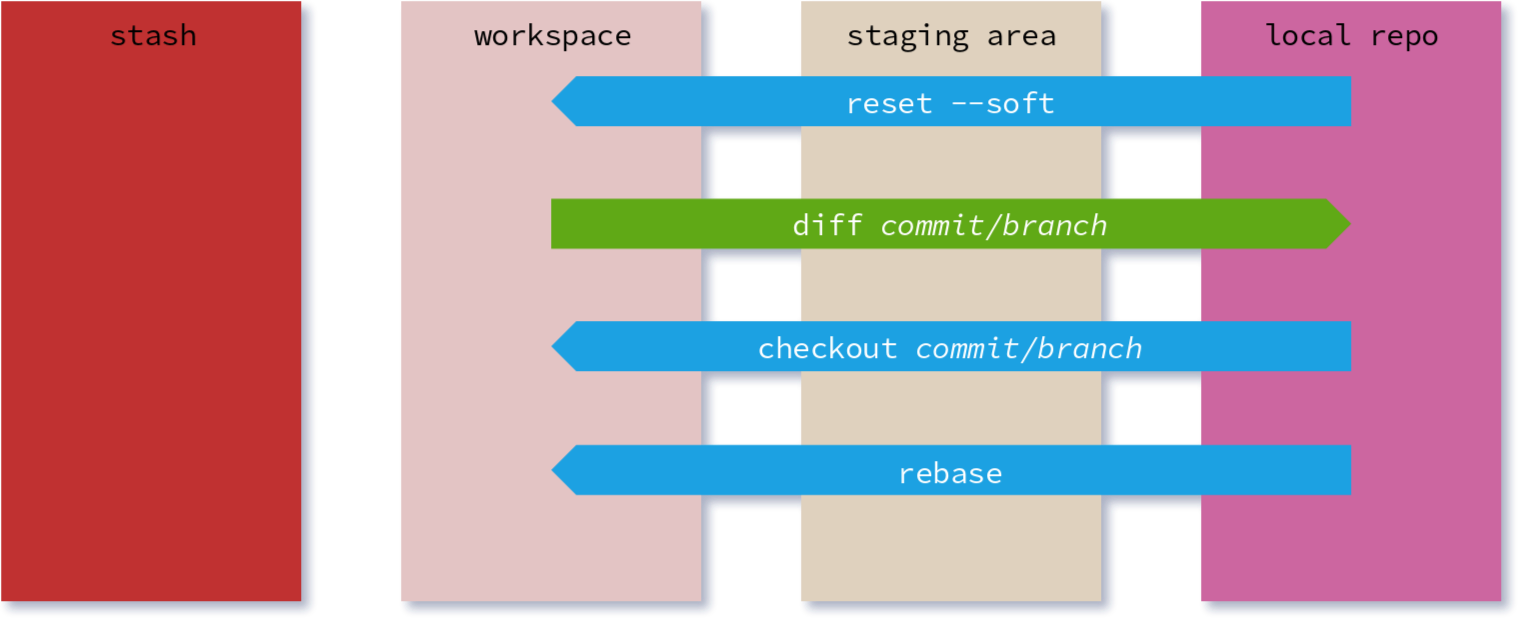
\includegraphics[width=1\textwidth,keepaspectratio]{./images/GitAreas-LocalRepo.png}
            }
            {
                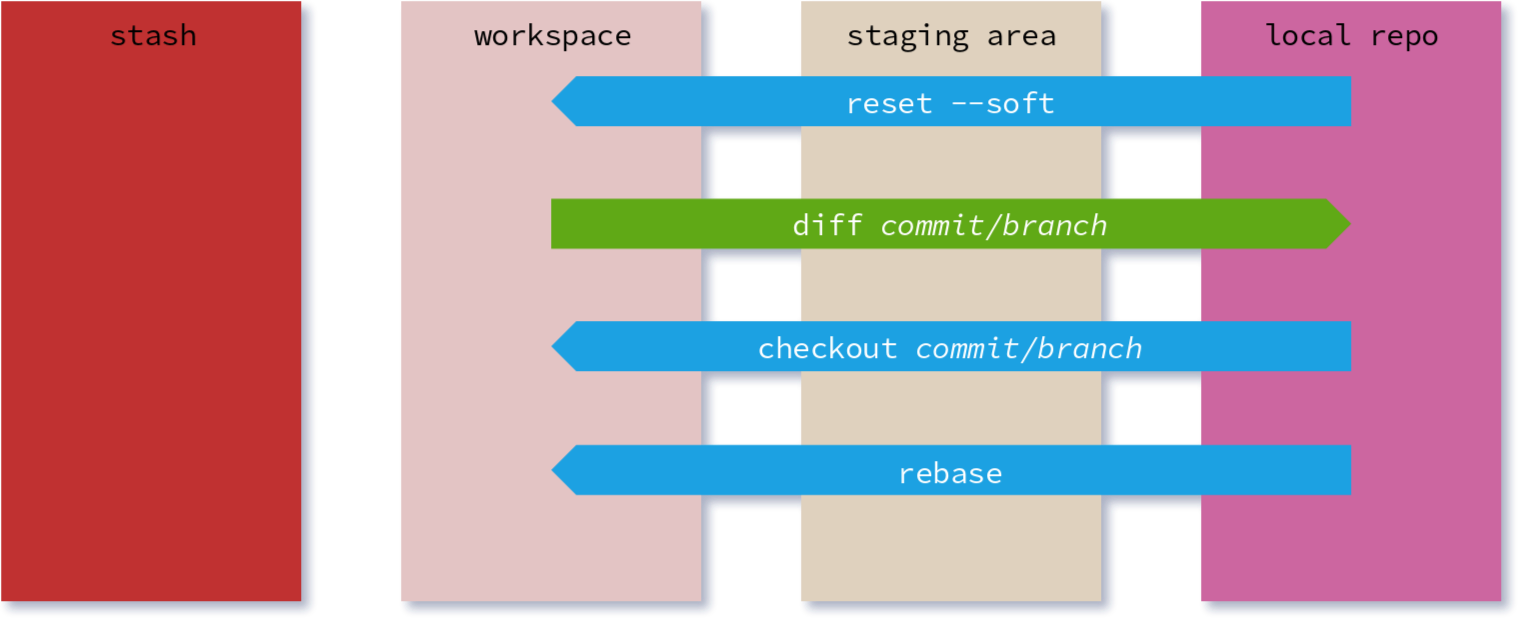
\includegraphics[height=0.75\textheight,keepaspectratio]{./images/GitAreas-LocalRepo.png}
            }
            \caption{Local repository area}
        \end{center}
    \end{figure}
\end{frame}

